% Options for packages loaded elsewhere
\PassOptionsToPackage{unicode}{hyperref}
\PassOptionsToPackage{hyphens}{url}
%
\documentclass[
]{article}
\usepackage{amsmath,amssymb}
\usepackage{iftex}
\ifPDFTeX
  \usepackage[T1]{fontenc}
  \usepackage[utf8]{inputenc}
  \usepackage{textcomp} % provide euro and other symbols
\else % if luatex or xetex
  \usepackage{unicode-math} % this also loads fontspec
  \defaultfontfeatures{Scale=MatchLowercase}
  \defaultfontfeatures[\rmfamily]{Ligatures=TeX,Scale=1}
\fi
\usepackage{lmodern}
\ifPDFTeX\else
  % xetex/luatex font selection
\fi
% Use upquote if available, for straight quotes in verbatim environments
\IfFileExists{upquote.sty}{\usepackage{upquote}}{}
\IfFileExists{microtype.sty}{% use microtype if available
  \usepackage[]{microtype}
  \UseMicrotypeSet[protrusion]{basicmath} % disable protrusion for tt fonts
}{}
\makeatletter
\@ifundefined{KOMAClassName}{% if non-KOMA class
  \IfFileExists{parskip.sty}{%
    \usepackage{parskip}
  }{% else
    \setlength{\parindent}{0pt}
    \setlength{\parskip}{6pt plus 2pt minus 1pt}}
}{% if KOMA class
  \KOMAoptions{parskip=half}}
\makeatother
\usepackage{xcolor}
\usepackage[margin=1in]{geometry}
\usepackage{graphicx}
\makeatletter
\def\maxwidth{\ifdim\Gin@nat@width>\linewidth\linewidth\else\Gin@nat@width\fi}
\def\maxheight{\ifdim\Gin@nat@height>\textheight\textheight\else\Gin@nat@height\fi}
\makeatother
% Scale images if necessary, so that they will not overflow the page
% margins by default, and it is still possible to overwrite the defaults
% using explicit options in \includegraphics[width, height, ...]{}
\setkeys{Gin}{width=\maxwidth,height=\maxheight,keepaspectratio}
% Set default figure placement to htbp
\makeatletter
\def\fps@figure{htbp}
\makeatother
\setlength{\emergencystretch}{3em} % prevent overfull lines
\providecommand{\tightlist}{%
  \setlength{\itemsep}{0pt}\setlength{\parskip}{0pt}}
\setcounter{secnumdepth}{-\maxdimen} % remove section numbering
\usepackage{caption}
\captionsetup[table]{labelformat=empty}
\usepackage[utf8]{inputenc}
\usepackage[spanish]{babel}
\usepackage{graphicx}
\usepackage{multirow,rotating}
\pagenumbering{gobble}
\usepackage{dcolumn}
\usepackage{booktabs}
\usepackage{longtable}
\usepackage{array}
\usepackage{multirow}
\usepackage{wrapfig}
\usepackage{float}
\usepackage{colortbl}
\usepackage{pdflscape}
\usepackage{tabu}
\usepackage{threeparttable}
\usepackage{threeparttablex}
\usepackage[normalem]{ulem}
\usepackage{makecell}
\usepackage{xcolor}
\ifLuaTeX
  \usepackage{selnolig}  % disable illegal ligatures
\fi
\IfFileExists{bookmark.sty}{\usepackage{bookmark}}{\usepackage{hyperref}}
\IfFileExists{xurl.sty}{\usepackage{xurl}}{} % add URL line breaks if available
\urlstyle{same}
\hypersetup{
  hidelinks,
  pdfcreator={LaTeX via pandoc}}

\author{}
\date{\vspace{-2.5em}}

\begin{document}

\begin{titlepage}
	
	\newcommand{\HRule}{\rule{\linewidth}{0.5mm}} % Defines a new command for the horizontal lines, change thickness here
	
	\center % Center everything on the page
	
	
\includegraphics[]{logoFC_UNAM.png}\\ % Include a department/university logo - this will require the graphicx package
	%----------------------------------------------------------------------------------------
	%	HEADING SECTIONS
	%----------------------------------------------------------------------------------------
	
	\hspace*{2cm}

	%\textsc{\Large Econometría}\\[1cm] % Major heading such as course name
	\textsc{\large  Análisis Multivariado}\\[1.5cm] 
	
	%----------------------------------------------------------------------------------------
	%	TITLE SECTION
	%----------------------------------------------------------------------------------------
	
	\HRule \\[0.4cm]
	{ \Large \bfseries Práctica 2}\\[0.4cm] % Title of your document
	\textsc{\Large Multicolinealidad, componentes principales, normal multivariado, proporción de varianzas, Biplot y regresión lineal múltiple.}\\[1cm] % Major heading such as course name
	\HRule \\[1.2cm]
	
	%----------------------------------------------------------------------------------------
	%	AUTHOR SECTION
	%----------------------------------------------------------------------------------------
	
	\begin{minipage}{0.4\textwidth}
		\begin{flushleft} \large
			\emph{}\\
Enríquez Hernández Leobardo\\
Tlahuiz Tenorio Saúl \\
		\end{flushleft}
	\end{minipage}
	~

	~
	% If you don't want a supervisor, uncomment the two lines below and remove the section above
	%\Large \emph{Author:}\\
	%John \textsc{Smith}\\[3cm] % Your name
	
	%----------------------------------------------------------------------------------------
	%	DATE SECTION
	%----------------------------------------------------------------------------------------
	
	{\today}\\[2cm] % Date, change the \today to a set date if you want to be precise
	
	%----------------------------------------------------------------------------------------
	%	LOGO SECTION
	%----------------------------------------------------------------------------------------
	

	
	%----------------------------------------------------------------------------------------
	
	\vfill % Fill the rest of the page with whitespace
	
\end{titlepage}

{
\setcounter{tocdepth}{3}
\tableofcontents
}
\pagenumbering{gobble}
\pagenumbering{arabic}

Utilizando la base de datos Student-Scores y con las columnas de las
calificaciones obtenidas por los alumnos realizaremos algunos análisis
de multicolinealidad de covariables, componentes principales, pruebas de
distribución normal multivariado, diagrama de dispersión y proporción de
varianza, el Biplot y agrupaciones, verificación de variables
importantes, y regresión lineal múltiple.

\hypertarget{anuxe1lisis-exploratorio-de-datos.}{%
\subsection{1. Análisis exploratorio de
datos.}\label{anuxe1lisis-exploratorio-de-datos.}}

Antes de comenzar cargamos la base de datos que vamos a utilizar y
hacemos una inspección rápida del tipo de datos para cada variable y de
la estadística descriptiva de los datos numéricos.

\begin{verbatim}
##        id          first_name         last_name            email          
##  Min.   :   1.0   Length:2000        Length:2000        Length:2000       
##  1st Qu.: 500.8   Class :character   Class :character   Class :character  
##  Median :1000.5   Mode  :character   Mode  :character   Mode  :character  
##  Mean   :1000.5                                                           
##  3rd Qu.:1500.2                                                           
##  Max.   :2000.0                                                           
##     gender          part_time_job       absence_days   
##  Length:2000        Length:2000        Min.   : 0.000  
##  Class :character   Class :character   1st Qu.: 2.000  
##  Mode  :character   Mode  :character   Median : 3.000  
##                                        Mean   : 3.666  
##                                        3rd Qu.: 5.000  
##                                        Max.   :10.000  
##  extracurricular_activities weekly_self_study_hours career_aspiration 
##  Length:2000                Min.   : 0.00           Length:2000       
##  Class :character           1st Qu.: 5.00           Class :character  
##  Mode  :character           Median :18.00           Mode  :character  
##                             Mean   :17.76                             
##                             3rd Qu.:28.00                             
##                             Max.   :50.00                             
##    math_score     history_score    physics_score    chemistry_score
##  Min.   : 40.00   Min.   : 50.00   Min.   : 50.00   Min.   : 50    
##  1st Qu.: 77.00   1st Qu.: 69.75   1st Qu.: 71.00   1st Qu.: 69    
##  Median : 87.00   Median : 82.00   Median : 83.00   Median : 81    
##  Mean   : 83.45   Mean   : 80.33   Mean   : 81.34   Mean   : 80    
##  3rd Qu.: 93.00   3rd Qu.: 91.00   3rd Qu.: 92.00   3rd Qu.: 91    
##  Max.   :100.00   Max.   :100.00   Max.   :100.00   Max.   :100    
##  biology_score    english_score   geography_score 
##  Min.   : 30.00   Min.   :50.00   Min.   : 60.00  
##  1st Qu.: 69.00   1st Qu.:72.00   1st Qu.: 71.00  
##  Median : 81.00   Median :83.00   Median : 81.00  
##  Mean   : 79.58   Mean   :81.28   Mean   : 80.89  
##  3rd Qu.: 91.00   3rd Qu.:91.00   3rd Qu.: 91.00  
##  Max.   :100.00   Max.   :99.00   Max.   :100.00
\end{verbatim}

Luego clasificaremos estas variables por escalas, agruparemos las
numéricas y enterios por un lado, luego las nominales y ordinales por
otro lado.

Ya que realizamos una inspección básica a las columnas de la base de
datos, el tipo de dato, así como sus estadísticos principales lo que
sigue será definir otras 2 variables donde tomaremos las columnas de las
calificaciones de los alumnos y otra con la variable dependiente para
hacer el modelo de regresión.

Con las nuevas variables definidas haremos un análisis exploratorio para
ver si no tendremos problemas de escalas con los datos, outliers, NA´s,
etc. Algo que debemos mencionar es que con la variable vars\_predict
donde guardamos las calificaciones de los alumnos no tendremos problemas
de escala ya que las calificaciones por alumno se encuentran definidas
con el mismo rango escalar de 0 a 100.

En los siguientes histogramas con BoxPlot y densidad combinados, podemos
observar algunos comportamientos de las variables explicativas. Por
ejemplo math\_score tiene una asimetría hacia la izquierda (o negativa),
mostrando varios outliers por debajo del primer cuantil. Por otro lado,
geography\_score muestra un comportamiento más uniforme, con mayor
simetría y sin outliers.

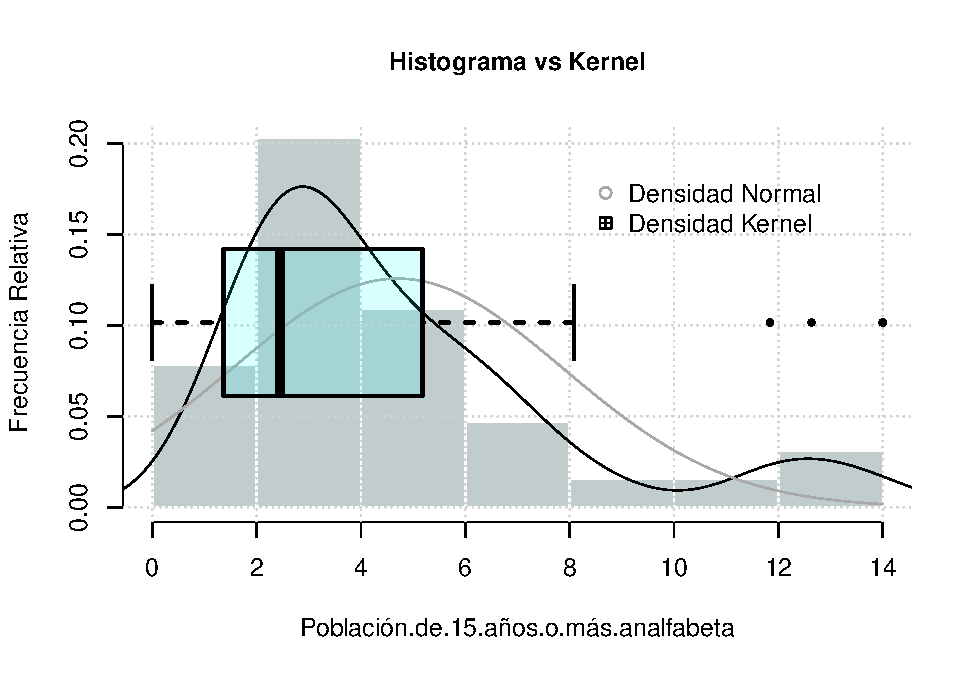
\includegraphics{Practica_2_files/figure-latex/unnamed-chunk-6-1.pdf}
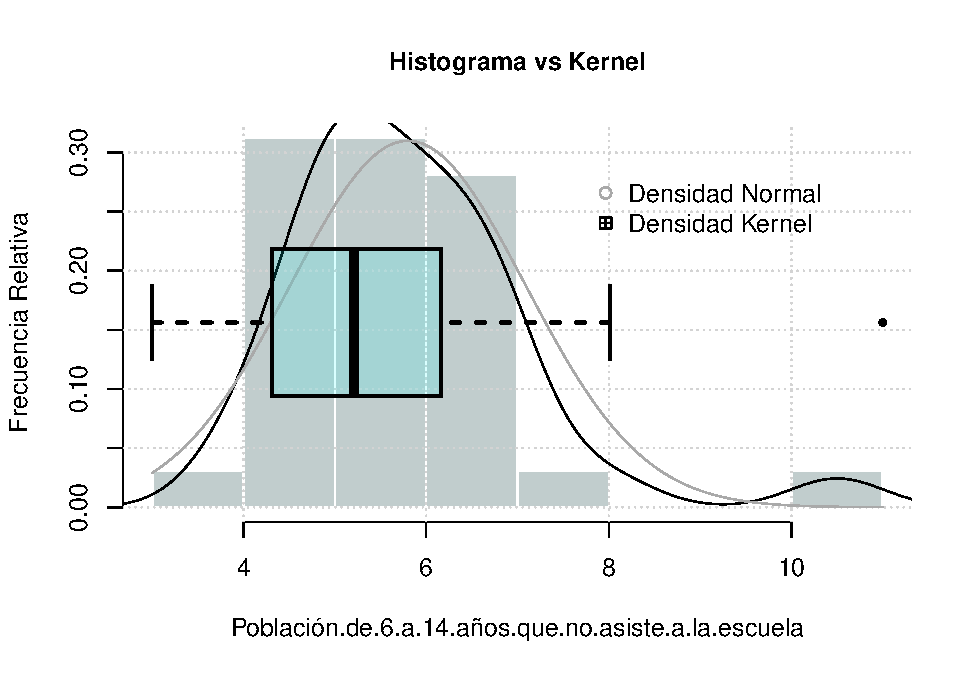
\includegraphics{Practica_2_files/figure-latex/unnamed-chunk-6-2.pdf}

En las siguientes gráficas de dispersión entre las covariables, podemos
observar que no hay relaciones lineales evidentes entre éstas.

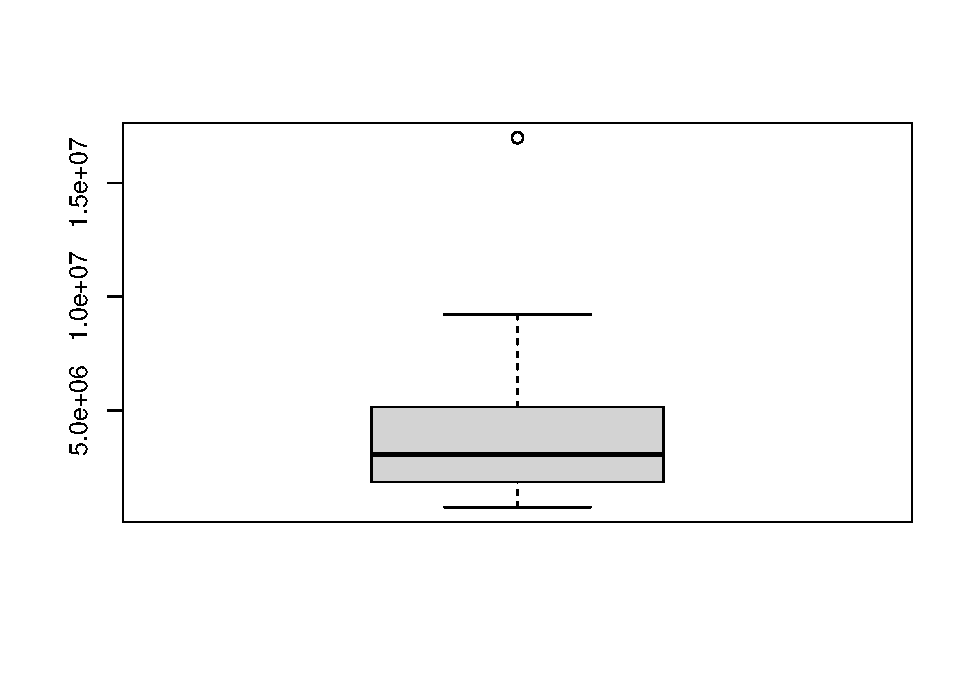
\includegraphics{Practica_2_files/figure-latex/unnamed-chunk-7-1.pdf}

En las siguientes gráficas de dispersión individuales, no se muestra
algún comportamiento, tendencia o patrón definido.

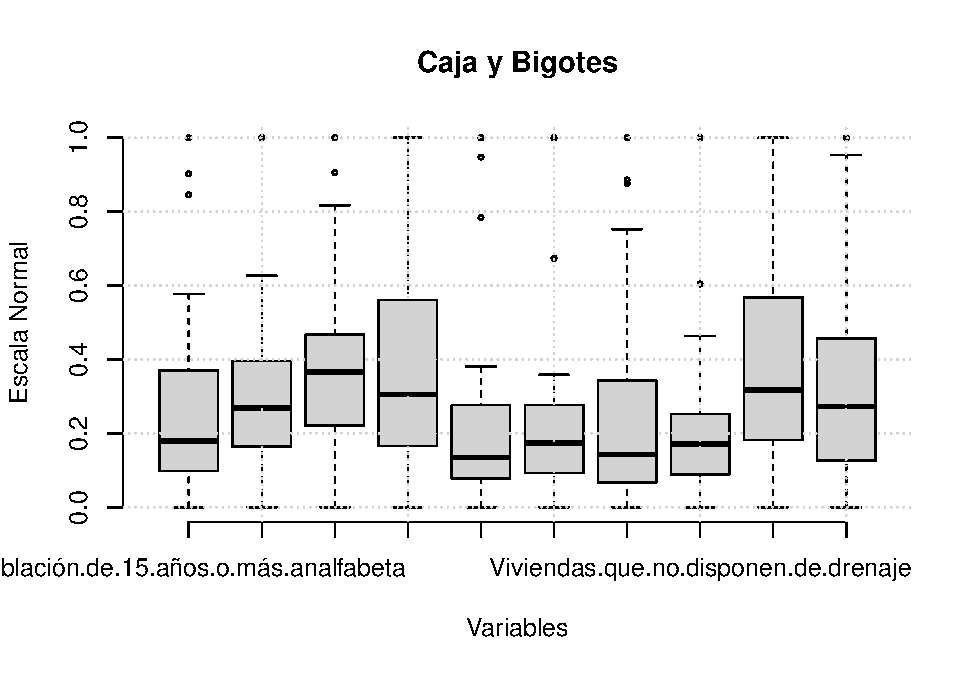
\includegraphics{Practica_2_files/figure-latex/unnamed-chunk-8-1.pdf}
\includegraphics{Practica_2_files/figure-latex/unnamed-chunk-8-2.pdf}

En los siguientes BoxPlot parece no haber problemas de escala, y algunos
aoutliers en las variables math\_score y biology\_score.

\includegraphics{Practica_2_files/figure-latex/unnamed-chunk-9-1.pdf}

Del análisis exploratorio que hicimos podemos ver que en efecto no
tenemos problemas de escala con las calificaciones, tenemos algunos
valores outliers o atípicos pero no es algo que nos genere problemas.

\hypertarget{determinar-si-existe-multicolinealidad-usando-vif-o-kmo.}{%
\subsection{2. Determinar si existe multicolinealidad usando VIF o
KMO.}\label{determinar-si-existe-multicolinealidad-usando-vif-o-kmo.}}

\begin{verbatim}
## Kaiser-Meyer-Olkin factor adequacy
## Call: KMO(r = student_scores[, vars_predict])
## Overall MSA =  0.66
## MSA for each item = 
##      math_score   history_score   physics_score chemistry_score   biology_score 
##            0.66            0.65            0.65            0.67            0.67 
##   english_score geography_score 
##            0.65            0.67
\end{verbatim}

De los resultados obtenidos de la prueba KMO tenemos que los valores son
mediocres o regulares para nuestras variables, pues están fuera del
rango 0.8 a 1, donde la muestra sería adecuada para el análisis
factorial. Sin embargo no son menores a 0.6, que indicaría que la
muestra no es adecuada.

Por otro lado, podemos observar el factor de inflación de varianza y
parece no haber multicolinealidad entre las covariables.

\begin{verbatim}
##                 Variance_Inflation_Factor
## math_score                       1.059224
## history_score                    1.055562
## physics_score                    1.047626
## chemistry_score                  1.051409
## biology_score                    1.046167
## english_score                    1.043667
## geography_score                  1.027365
\end{verbatim}

\hypertarget{componentes-principales}{%
\subsection{3. Componentes principales}\label{componentes-principales}}

Ahora obtendremos las componentes principales de nuestras variables
predictoras. Se observa que la proporción de varianza no se acumula
rápidamente a 1, el primer componente tiene 0.23, y los primeros tres
acumulan 0.52, es decir, la mitad. Hasta el quinto componente acumula
77\%.

\begin{verbatim}
## Importance of components:
##                            Comp.1     Comp.2     Comp.3     Comp.4     Comp.5
## Standard deviation     16.1894537 13.2037936 12.3394732 12.0545319 11.7906155
## Proportion of Variance  0.2328853  0.1549084  0.1352916  0.1291155  0.1235238
## Cumulative Proportion   0.2328853  0.3877937  0.5230853  0.6522008  0.7757246
##                            Comp.6     Comp.7
## Standard deviation     11.3260534 11.1413200
## Proportion of Variance  0.1139816  0.1102938
## Cumulative Proportion   0.8897062  1.0000000
\end{verbatim}

La matriz Gamma o de vectores propios es la siguiente.

\begin{verbatim}
## 
## Loadings:
##                 Comp.1 Comp.2 Comp.3 Comp.4 Comp.5 Comp.6 Comp.7
## math_score       0.455  0.490  0.218  0.547  0.404         0.207
## history_score    0.380  0.368 -0.500 -0.330 -0.207  0.563       
## physics_score    0.348 -0.195  0.589  0.137 -0.509  0.332 -0.327
## chemistry_score  0.401         0.368 -0.727  0.320 -0.268       
## biology_score    0.489 -0.712 -0.362  0.180  0.293              
## english_score    0.285  0.250 -0.299  0.107 -0.327 -0.644 -0.484
## geography_score  0.217 -0.127               -0.490 -0.291  0.782
## 
##                Comp.1 Comp.2 Comp.3 Comp.4 Comp.5 Comp.6 Comp.7
## SS loadings     1.000  1.000  1.000  1.000  1.000  1.000  1.000
## Proportion Var  0.143  0.143  0.143  0.143  0.143  0.143  0.143
## Cumulative Var  0.143  0.286  0.429  0.571  0.714  0.857  1.000
\end{verbatim}

La muestra aleatoria de las componentes principales es la siguiente, se
muestran las primeras 10.

\begin{verbatim}
##            Comp.1      Comp.2      Comp.3     Comp.4     Comp.5    Comp.6
##  [1,]  -0.7618592   3.9668266  16.9228253 -19.763332 -12.299268 -2.028698
##  [2,]  27.2381257  -3.9896721   8.8395286  -8.133651  -3.200276 -3.822412
##  [3,]  10.8878736  10.2934527  11.6784544 -19.563597 -15.583157  8.038332
##  [4,]  -5.2530396 -21.6573752   6.4468393  -4.023467  -0.870790  8.953877
##  [5,] -15.6437646   0.3758993 -11.3431384   9.306846   9.325239  2.860983
##  [6,]   2.6354894  19.3433696 -13.7773673  -3.262716   3.103894  6.729581
##  [7,]  14.6028988   4.9981457   0.6833324  11.341741   5.301996 24.818274
##  [8,]   4.0685963   4.0334681  -8.8920743  13.544673  -1.177618 19.489528
##  [9,]   3.2070066  -3.4125735  19.3950023   7.330242   9.122398  3.460563
## [10,]  -9.7758235   8.8484338  17.0498812  15.711055   5.489164  7.068756
##            Comp.7
##  [1,]   0.3967555
##  [2,]   0.0857024
##  [3,]   8.8575581
##  [4,]   7.2897149
##  [5,]   4.9865151
##  [6,]  10.9458277
##  [7,] -12.4114245
##  [8,]  11.1719512
##  [9,]  -5.9750084
## [10,]  -0.1306289
\end{verbatim}

\hypertarget{distribucion-normal-multivariado.}{%
\subsection{4. Distribucion Normal
multivariado.}\label{distribucion-normal-multivariado.}}

Con las componentes obtenidas veremos si estas se distribuyen de forma
normal multivariada con el Henze-Zirkler's test y el método de detección
de outliers quan que es un método cuantil basado en la distancia
Mahalanobis. A continuación se muestra el Chi-Square Q-Q Plot generado.

\includegraphics{Practica_2_files/figure-latex/unnamed-chunk-15-1.pdf}

Observemos que el test de Henze-Zirkler rechaza que sea normal
multivariado.

\begin{verbatim}
##            Test       HZ p value MVN
## 1 Henze-Zirkler 3.050838       0  NO
\end{verbatim}

Finalmente, el test de Anderson-Darling muestra que para 5 de los 7
componentes no forman una normal multivariada, particularmente las
primeras dos componentes que nos interesan.

\begin{verbatim}
##               Test  Variable Statistic   p value Normality
## 1 Anderson-Darling   comp1      2.3329  <0.001      NO    
## 2 Anderson-Darling   comp2      1.4887   8e-04      NO    
## 3 Anderson-Darling   comp3      0.2034  0.8765      YES   
## 4 Anderson-Darling   comp4      1.2723  0.0026      NO    
## 5 Anderson-Darling   comp5      0.5219   0.184      YES   
## 6 Anderson-Darling   comp6      1.1058  0.0067      NO    
## 7 Anderson-Darling   comp7      0.8082  0.0365      NO
\end{verbatim}

\hypertarget{diagrama-de-dispersion-y-proporciuxf3n-de-varianza.}{%
\subsection{5. Diagrama de Dispersion y proporción de
varianza.}\label{diagrama-de-dispersion-y-proporciuxf3n-de-varianza.}}

Con la variable de scores obtenida del calculo de las componentes
principales graficaremos un diagrama de dispersión tomando únicamente
las primeras 2 componentes. Lo que podemos observar es que las primeras
2 componentes no están conservando mucha variabilidad de los datos
originales.

\includegraphics{Practica_2_files/figure-latex/unnamed-chunk-18-1.pdf}

Si graficamos los primeros tres componentes tenemos lo siguiente.

\includegraphics{Practica_2_files/figure-latex/unnamed-chunk-19-1.pdf}

\hypertarget{biplot-agrupaciones-y-variables-importantes.}{%
\subsection{6. Biplot, agrupaciones y variables
importantes.}\label{biplot-agrupaciones-y-variables-importantes.}}

En la siguiente gráfica Biplot de los primeros dos componentes vemos las
flechas que son las variables y los puntos numéricos que son las
observaciones. El largo de las flechas indica la varianza, entre más
largas mayor varianza. El coseno del ángulo entre las flechas aproxima
la correlación entre las variables, entre más cercano a 90 o 270 grados
menor correlación entre las variables, un ángulo de 0 o de 180 grados
refleja correlación de 1 y -1 respectivamente. Observamos aquí las
correlaciones entre las variables dentro de los componentes principales.

\includegraphics{Practica_2_files/figure-latex/unnamed-chunk-20-1.pdf}

Por otro lado, podemos usar otro método, en el que en ncp indicamos el
número de componentes principales que queremos, y con ello obtenemos un
PCA graph, por una parte de observaciones y por otro de la variable, por
separado.

\includegraphics{Practica_2_files/figure-latex/unnamed-chunk-21-1.pdf}
\includegraphics{Practica_2_files/figure-latex/unnamed-chunk-21-2.pdf}

Para determinar la importancia de cada componente con las variables
originales usaremos la función cos2 la cual nos dice que un valor bajo
significa que la variable no está perfectamente representada por esa
componente, mientras que un valor alto significa que es una buena
representación de esa varíable con esa componente. con Coseno 2 podemos
observar la importancia de las variables en las primeras componentes
principales. En este caso tenemos las correlaciones entre las variables
y las componentes principales.

\includegraphics{Practica_2_files/figure-latex/unnamed-chunk-22-1.pdf}

Observando las dimensiones tenemos lo siguiente.

\begin{verbatim}
## 
## Link between the variable and the continuous variables (R-square)
## =================================================================================
##                 correlation       p.value
## math_score        0.5277368 7.999187e-144
## chemistry_score   0.5088131 3.603752e-132
## history_score     0.5017574 5.212873e-128
## biology_score     0.4812949 1.757672e-116
## physics_score     0.4687030 9.099105e-110
## english_score     0.4540056 2.806852e-102
## geography_score   0.3803661  7.369194e-70
\end{verbatim}

\begin{verbatim}
## 
## Link between the variable and the continuous variables (R-square)
## =================================================================================
##                 correlation       p.value
## physics_score    0.47086177 6.726618e-111
## geography_score  0.38903172  2.900618e-73
## biology_score    0.37711742  1.310961e-68
## chemistry_score  0.09926032  8.696948e-06
## math_score      -0.30379176  5.706193e-44
## history_score   -0.45669936 1.267281e-103
## english_score   -0.46520160 5.978037e-108
\end{verbatim}

Otra forma de visualizar esto es combinar el biplot y la importancia de
las componentes en el que los atributos con puntuaciones cos2 similares
tendrán colores similares.

\includegraphics{Practica_2_files/figure-latex/unnamed-chunk-24-1.pdf}

\hypertarget{regresiuxf3n-lineal-muxfaltiple.-modelo-predictivo.}{%
\subsection{7. Regresión lineal múltiple. Modelo
predictivo.}\label{regresiuxf3n-lineal-muxfaltiple.-modelo-predictivo.}}

Como ultimo paso ajustaremos un modelo de regresión usando las variables
que definimos al principio donde tomamos las calificaciones y la
variable que nos interesa modelar.

Se muestra a continuación el factor de inflación de varianza para un
modelo de regresión con datos originales, todos son cercanos a 1 por lo
que no parece haber problemas de multicolinealidad.

\begin{verbatim}
##                 Variance_Inflation_Factor
## math_score                       1.059224
## history_score                    1.055562
## physics_score                    1.047626
## chemistry_score                  1.051409
## biology_score                    1.046167
## english_score                    1.043667
## geography_score                  1.027365
\end{verbatim}

A continuación se muestra el summary del modelo ajustado con los datos
originales.

\begin{verbatim}
## 
## Call:
## lm(formula = weekly_self_study_hours ~ ., data = datos)
## 
## Residuals:
##      Min       1Q   Median       3Q      Max 
## -26.8797  -7.5630   0.3167   8.0106  24.8864 
## 
## Coefficients:
##                  Estimate Std. Error t value Pr(>|t|)    
## (Intercept)     -62.86002    3.12556 -20.112  < 2e-16 ***
## math_score        0.28307    0.01790  15.815  < 2e-16 ***
## history_score     0.16762    0.01855   9.034  < 2e-16 ***
## physics_score     0.11099    0.01877   5.912 3.96e-09 ***
## chemistry_score   0.09286    0.01846   5.031 5.32e-07 ***
## biology_score     0.09042    0.01714   5.274 1.48e-07 ***
## english_score     0.15483    0.01954   7.925 3.76e-15 ***
## geography_score   0.09015    0.02003   4.501 7.17e-06 ***
## ---
## Signif. codes:  0 '***' 0.001 '**' 0.01 '*' 0.05 '.' 0.1 ' ' 1
## 
## Residual standard error: 10.28 on 1992 degrees of freedom
## Multiple R-squared:  0.2838, Adjusted R-squared:  0.2813 
## F-statistic: 112.8 on 7 and 1992 DF,  p-value: < 2.2e-16
\end{verbatim}

A continuación mostramos el factor de inflación de varianza para un
modelo de regresión con componentes principales, todos son 1 por lo que
no hay problemas de multicolinealidad.

\begin{verbatim}
##       Variance_Inflation_Factor
## comp1                         1
## comp2                         1
## comp3                         1
## comp4                         1
## comp5                         1
## comp6                         1
## comp7                         1
\end{verbatim}

A continuación se presenta el summary del modelo ajustando con los
componentes principales.

\begin{verbatim}
## 
## Call:
## lm(formula = weekly_self_study_hours ~ ., data = data2)
## 
## Residuals:
##      Min       1Q   Median       3Q      Max 
## -26.8797  -7.5630   0.3167   8.0106  24.8864 
## 
## Coefficients:
##              Estimate Std. Error t value Pr(>|t|)    
## (Intercept) 17.755500   0.229940  77.218  < 2e-16 ***
## comp1        0.376119   0.014203  26.481  < 2e-16 ***
## comp2        0.143781   0.017415   8.256 2.70e-16 ***
## comp3       -0.001283   0.018635  -0.069    0.945    
## comp4        0.081004   0.019075   4.247 2.27e-05 ***
## comp5       -0.015468   0.019502  -0.793    0.428    
## comp6       -0.010707   0.020302  -0.527    0.598    
## comp7        0.019595   0.020639   0.949    0.343    
## ---
## Signif. codes:  0 '***' 0.001 '**' 0.01 '*' 0.05 '.' 0.1 ' ' 1
## 
## Residual standard error: 10.28 on 1992 degrees of freedom
## Multiple R-squared:  0.2838, Adjusted R-squared:  0.2813 
## F-statistic: 112.8 on 7 and 1992 DF,  p-value: < 2.2e-16
\end{verbatim}

\end{document}
